\section{分析結果}
実験後,分析を行った結果,テスト2,3ではフィードバック利用回数が減少したとともに,テスト1,3の統制群にあった外れ値が実験群ではなくなった.
ポストテストの結果,統制群に比べ実験群の方が点数が高くなったことを図に示す.T検定の結果,p<0.1となったため,有意傾向にあることが分かった.

\begin{figure}[tb]
	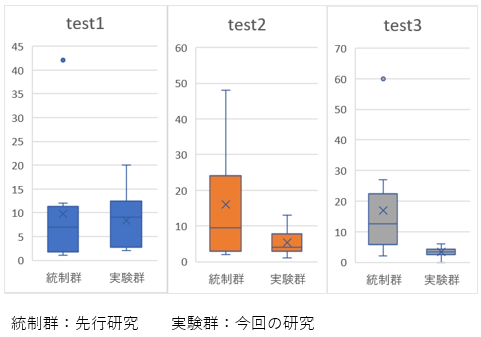
\includegraphics[width=0.9\linewidth]{tex1.png}
	\centering
	\caption{フィードバック利用回数}
	\label{fig1}
\end{figure}